\documentclass{beamer}
\usepackage[serbianc]{babel}
\usepackage{graphicx}
\usepackage{makeidx}
\hypersetup{unicode}
\makeindex
\usefonttheme{professionalfonts}
\usetheme{CambridgeUS}

\title{Основе веб програмирања}
\author{Борисав Живановић (borisavz)}

\begin{document}

    \begin{frame}
        \maketitle
    \end{frame}

    \begin{frame}{Садржај}
        \begin{enumerate}
            \item Основни појмови мрежног програмирања
            \item Клијент-сервер архитектура
            \item Еволуција веб апликација
            \item HTTP протокол
            \item Рад са базом података
            \item Архитектура веб апликације
            \item Аутентификација и ауторизација
        \end{enumerate}
    \end{frame}

    \section{Основни појмови мрежног програмирања}
    \subsection{Packet switching}

    \begin{frame}[allowframebreaks]{Packet switching}
        \begin{itemize}
            \item Потребно је да поруку пошаљемо примаоцу
            \item Директна веза са сваким примаоцем није остварива
            \item Идеја: повезивање пошиљаоца/примаоца у мрежу, дељење комуникационог канала
            \item Решење: \textbf{комутација пакета (packet switching)}
            \begin{itemize}
                \item Поруку изделимо на пакете
                \item Пакетима додамо заглавље (header) са адресом пошиљаоца и примаоца
                \item Систем зна путање до примаоца
                \item Поруку шаљемо пакет по пакет
                \item Само један пакет заузима комуникациони канал
                \item Пакети могу да путују различитим путањама кроз мрежу, да дођу у различитом редоследу до примаоца, или да нестану
            \end{itemize}
        \end{itemize}

        \framebreak

        \begin{figure}
            \centering
            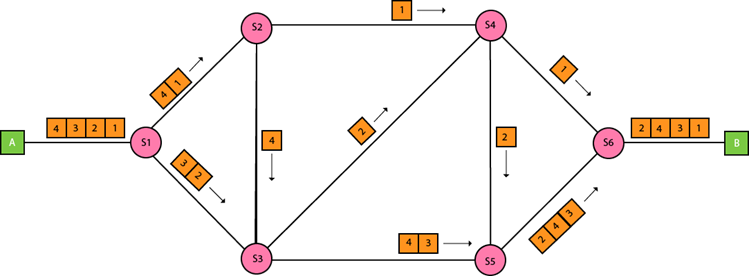
\includegraphics[width=0.75\textwidth]{images/pcsw.png}
            \caption{комутација пакета (packet switching)}
            \label{fig:pcsw}
        \end{figure}
    \end{frame}

    \subsection{IP, DNS}

    \begin{frame}[allowframebreaks]{Internet Protocol}
        \begin{itemize}
            \item Како би комуницирали у мрежи, потребно је да сваки учесник у комуникацији има додељену \textbf{јединствену} адресу
            \item Поруци придружујемо \textbf{заглавље (header)} које садржи:
            \begin{itemize}
                \item Адресу пошиљаоца (source address)
                \item Адресу примаоца (destination address)
                \item Додатна поља (верзија IP протокола, flags, TTL, checksum, ...)
            \end{itemize}
            \item Захваљујући овом заглављу систем зна коме да проследи поруку
            \item У одговори су адресе пошиљаоца и примаоца \textbf{замењене}!
        \end{itemize}

        \framebreak

        \begin{figure}
            \centering
            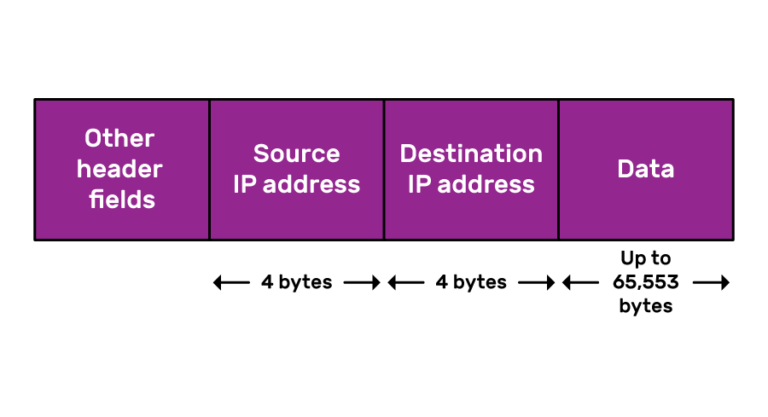
\includegraphics[width=0.75\textwidth]{images/ip.png}
            \caption{упрошћена структура IP пакета}
            \label{fig:ip}
        \end{figure}
    \end{frame}

    \begin{frame}[allowframebreaks]{DNS}
        \begin{itemize}
            \item Проблем: све више сервера на мрежи
            \item Није практично памтити сваку адресу у бројчаном облику
            \item Идеја: систем за придруживање имена, сличан телефонском именику
            \item Решење: \textbf{DNS (Domain Name System)}
            \begin{itemize}
                \item IP адреси додељујемо симболичко име (домен)
                \item Домени су хијерархијски (структура стабла)
                \item DNS је одговоран за одређени део хијерархије
                \item Као одговор враћа IP адресу или адресу одговорног DNS сервера
                \item Морамо знати IP адресу DNS сервера!
            \end{itemize}
        \end{itemize}

        \framebreak

        \begin{figure}
            \centering
            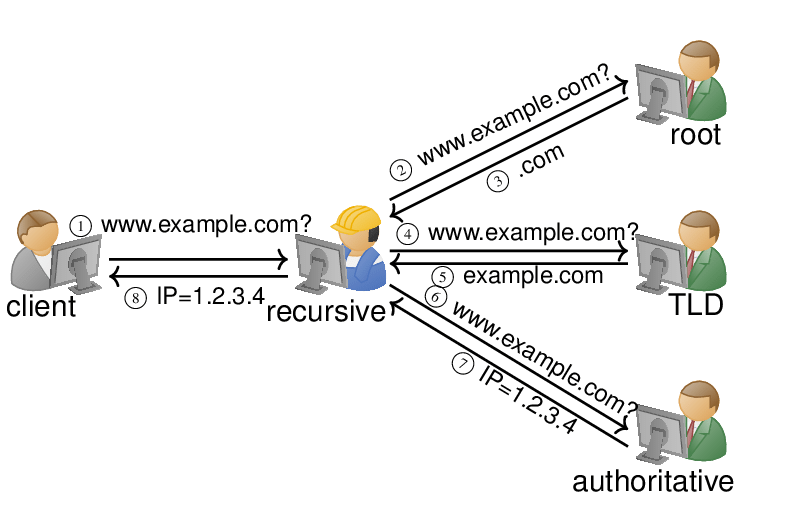
\includegraphics[width=0.75\textwidth]{images/dns.png}
            \caption{DNS упит}
            \label{fig:dns}
        \end{figure}
    \end{frame}
    
    \subsection{TCP, UDP}
    
    \begin{frame}[allowframebreaks]{Transmission Control Protocol}
        \begin{itemize}
            \item Решили смо проблем адресирања уређаја на мрежи...
            \item ...али нисмо проблеме редоследа пристиглих пакета и нестајања пакета
            \item Додатни проблем: шта ако имамо више мрежних апликација на истом рачунару, како да проследимо поруку одговарајућој апликацији?
        \end{itemize}
        
        \framebreak
        
        \begin{itemize}
            \item Решење: \textbf{TCP (Transmission Control Protocol)}
            \begin{itemize}
                \item Додајемо додатно заглавље на нашу поруку
                \item Заглавље садржи source и destination port (слично адреси пошиљаоца и примаоца, али се односи на апликацију), sequence number (редослед поруке)
                \item Уколико пакет нестане, шаље се поново
                \item Оперативни систем осигурава да само једна апликација користи одређени порт
            \end{itemize}
        \end{itemize}
        
        \framebreak
        
        \begin{figure}
            \centering
            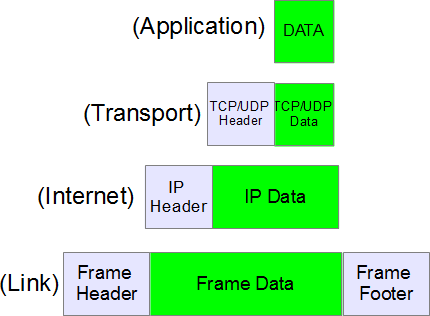
\includegraphics[width=0.6\textwidth]{images/enc.png}
            \caption{енкапсулација пакета}
            \label{fig:tcp_enc}
        \end{figure}
        
        \framebreak
        
        \begin{figure}
            \centering
            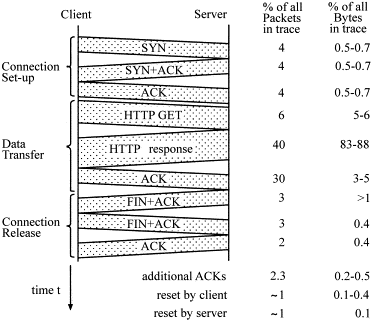
\includegraphics[width=0.5\textwidth]{images/tcp_http.png}
            \caption{Ток TCP комуникације}
            \label{fig:tcp_flow}
        \end{figure}
    \end{frame}
    
    \begin{frame}[allowframebreaks]{User Datagram Protocol}
        \begin{itemize}
            \item Успостављање конекције траје одређено време
            \item За поруке које стају у један пакет, можемо користити једноставнији \textbf{UDP (User Datagram Protocol)}
            \item Задржавамо адресирање апликација, али губимо гаранцију испоруке
            \item DNS користи UDP
            \item Омогућава изградњу протокола који имају гаранције испоруке
            \begin{itemize}
                \item пример: HTTP3/QUIC
            \end{itemize}
        \end{itemize}
    
        \framebreak
        
        \begin{figure}
            \centering
            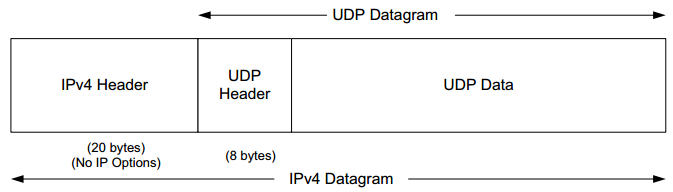
\includegraphics[width=0.75\textwidth]{images/udp_enc.png}
            \caption{енкапсулација пакета}
            \label{fig:udp_enc}
        \end{figure}
        
        \framebreak
        
        \begin{figure}
            \centering
            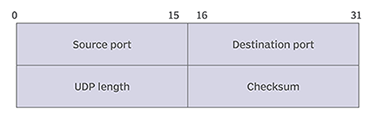
\includegraphics[width=0.75\textwidth]{images/udp_header.png}
            \caption{Садржај заглавља}
            \label{fig:udp_header}
        \end{figure}
    \end{frame}
    
    \section{Клијент-сервер архитектура}
    
    \begin{frame}{Однос између чворова}
        \begin{itemize}
            \item До сада смо говорили искључиво о чворовима који учествују у комуникацији
            \item Видели смо да један чвор започиње комуникацију, а други даје одговор
            \item У раду уочавамо две врсте односа између чворова:
            \begin{itemize}
                \item \textbf{peer-to-peer}: обе стране су подједнако важне у комуникацији
                \item \textbf{client-server}: клијент се обраћа серверу за податке или обављање акције
            \end{itemize}
        \end{itemize}
    \end{frame}
    
    \begin{frame}[allowframebreaks]{Клијент-сервер архитектура}
        \begin{itemize}
            \item Модел настао још раних дана рачунарства
            \item Рачунари су били велики и скупи
            \item Било је потребно омогућити дељење ресурса између више корисника
            \item Клијенти су били далеко једноставнији, главна намена је била слање команде и испис резултата
            \item Данас је овај приступ познат као \textbf{thin-client}
        \end{itemize}
        
        \framebreak
        
        \begin{figure}
            \centering
            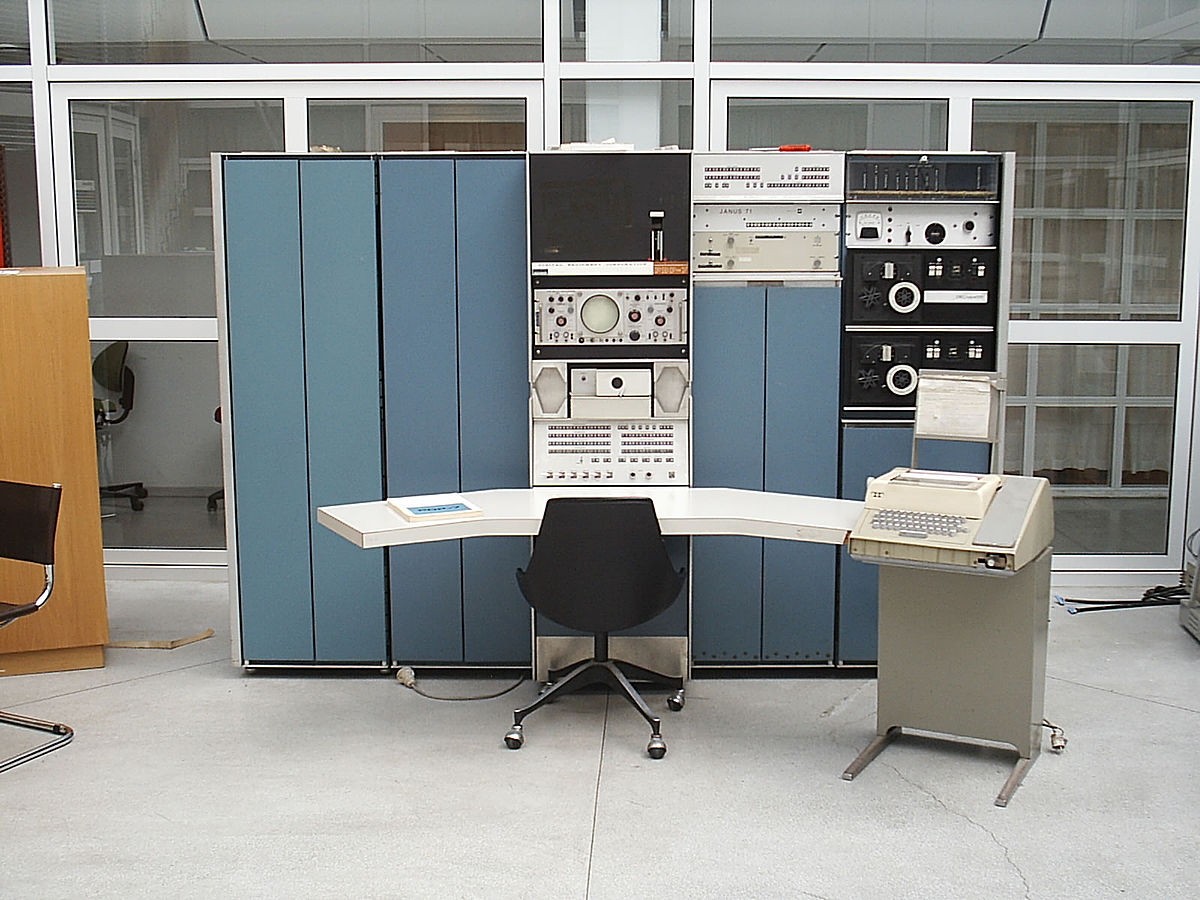
\includegraphics[width=0.65\textwidth]{images/pdp7.jpeg}
            \caption{PDP-7 (рачунар)}
            \label{fig:mainframe}
        \end{figure}
        
        \framebreak
        
        \begin{figure}
            \centering
            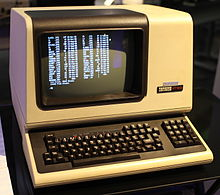
\includegraphics[width=0.5\textwidth]{images/DEC_VT100_terminal.jpg}
            \caption{DEC VT100 (терминал)}
            \label{fig:terminal}
        \end{figure}
        
        \framebreak
        
        \begin{itemize}
            \item Кроз године, рачунарска моћ је расла
            \item Ово је довело до појаве \textbf{PC (Personal Computer)}
            \begin{itemize}
                \item користи се непосредно
                \item без конукурентних корисничких сесија
            \end{itemize}
            \item Потреба за централним сервером и даље није потпуно избачена, али је могућа далеко већа интерактивност
            \item Данас је овај приступ познат као \textbf{thick-client}
            \begin{itemize}
                \item пример: Google Docs
            \end{itemize}
        \end{itemize}
    \end{frame}
    
    \section{Еволуција веб апликација}
    
    \begin{frame}[allowframebreaks]{Еволуција веб апликација}
        \begin{itemize}
            \item \textbf{World Wide Web (WWW)} је изумео Тим Бернерс-Ли у CERN-у
            \item Оригинална замисао је била систем за дељење докумената
            \item Језик докумената: \textbf{HTML (HyperText Markup Language)}
            \item Протокол за комуникацију: \textbf{HTTP (HyperText Transfer Protocol)}
            \item Иницијално садржај је био статички (могуће је прегледање искључиво предефинисаних докумената)
            \item Убрзо су уочени недостаци и настала је потреба за динамичким садржајем
        \end{itemize}
        
        \framebreak
        
        \begin{itemize}
            \item Идеја: чувати садржај у бази података и на основу њега динамички генерисати HTML документе
            \item Постоје два решења:
            \begin{itemize}
                \item \textbf{server-side render}: HTML документ генеришемо користећи шаблон и вредности из базе података
                \item \textbf{client-side render}: са сервера учитавамо основни HTML и JavaScript код, након тога размењујемо JSON објекте
            \end{itemize}
        \end{itemize}
        
        \framebreak
        
        \begin{figure}
            \centering
            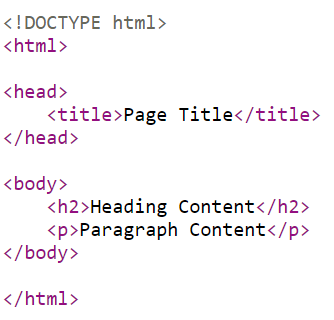
\includegraphics[width=0.5\textwidth]{images/html.png}
            \caption{HTML документ}
            \label{fig:html}
        \end{figure}
        
        \framebreak
        
        \begin{figure}
            \centering
            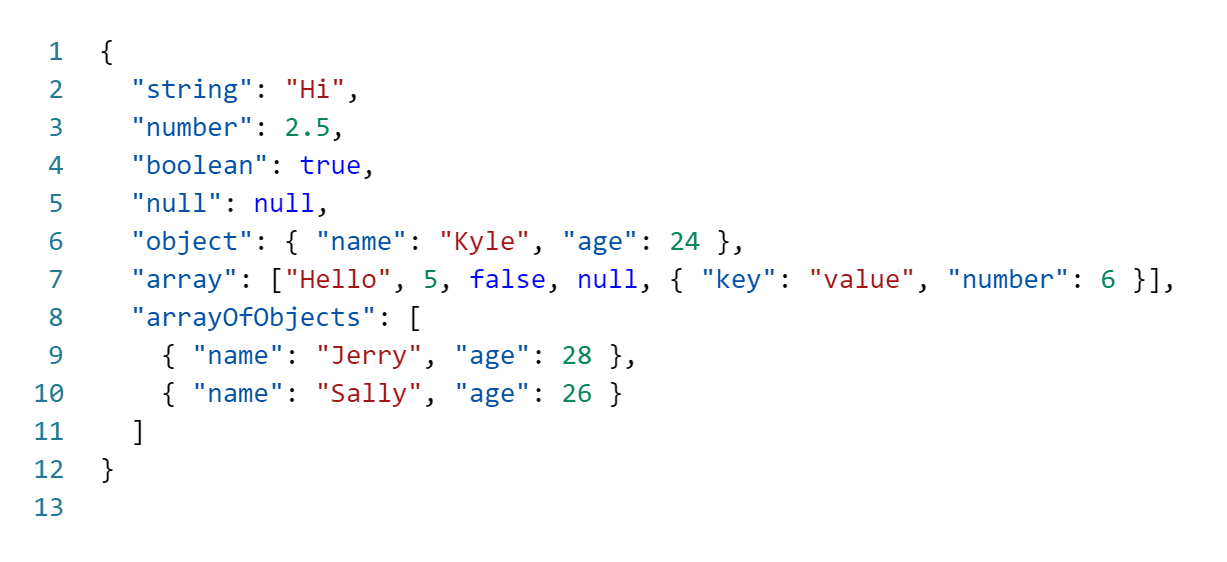
\includegraphics[width=0.5\textwidth]{images/json.png}
            \caption{JSON објекат}
            \label{fig:json}
        \end{figure}
    \end{frame}
    
    \section{HTTP протокол}
    
    \begin{frame}{HTTP протокол}
        \begin{itemize}
            \item Основни појмови мрежног програмирања
        \end{itemize}
    \end{frame}
\end{document}
